\documentclass[12pt]{report}
\usepackage{graphicx}
\usepackage[utf8]{vietnam}
\usepackage[left=2cm, right=2cm, top=2cm, bottom=2cm]{geometry}
\usepackage{subfiles}
\usepackage{fancyhdr}
\usepackage{hyperref}
\usepackage{etoolbox}
\usepackage{float}
\usepackage{amsmath}
\usepackage{array}
\usepackage{multirow}
\usepackage{booktabs}
\newcommand{\tabitem}{~~\llap{\textbullet}~~}

\usepackage[nottoc,notlof,notlot]{tocbibind} 
\renewcommand\bibname{References}

% Link color setup
\hypersetup{
	colorlinks = true,
	linkcolor = black,
	citecolor = blue
}

% Change format of page
\pagestyle{fancy}
\fancyhf{}
\fancyhead{}
\fancyfoot{}
\fancyhead[L]{Phân tích và thiết kế hệ thống thông tin}
\fancyfoot[L]{Hệ thống quản lý thư viện}
\fancyfoot[R]{\thepage}
\renewcommand{\headrulewidth}{1pt}
\renewcommand{\footrulewidth}{1pt}

\renewcommand{\thesection}{\arabic{section}}
\renewcommand{\thesubsection}{\thesection.\arabic{subsection}}
\renewcommand{\thesubsubsection}{\thesubsection.\arabic{subsubsection}}

% format
\usepackage{titlesec}
\usepackage{etoolbox}
\makeatletter
\patchcmd{\ttlh@hang}{\parindent\z@}{\parindent\z@\leavevmode}{}{}
\patchcmd{\ttlh@hang}{\noindent}{}{}{}
\makeatother

\titleformat{\subsection}
{\normalfont\large\bfseries}{\thesubsection}{1em}{}
\titleformat{\subsubsection}
{\normalfont\large\sffamily\bfseries}{\thesubsubsection}{1em}{}

% tab command
\newcommand\tab[1][1cm]{\hspace*{#1}}

\begin{document}

\subfile{sections/title-page.tex}

\pagenumbering{gobble}
\tableofcontents 
\newpage

\pagenumbering{arabic}
\newpage
\setcounter{page}{1}

\section{Giới thiệu đề tài}
Ngày nay, nguồn tri thức đang không ngừng tăng thêm và lượng thông tin của con người mở rộng một cách nhanh chóng, 
kéo theo đó là nhu cầu đọc và tra cứu tài liệu của con người cũng tăng theo rõ rệt. 
Để đáp ứng nhu cầu đó, các hệ thống hỗ trợ người đọc, tiêu biểu như thư viện, cần được nâng cấp, 
sửa đổi và cải tiến. Trong khi đó, các hệ thống thông tin lại đang cho thấy rất nhiều ưu điểm. 
Trong bài này, chúng em xin trình bày về một hệ thống thông tin thư viện và quá trình xây dựng nó.

\section{Yêu cầu hệ thống}
\subfile{sections/system-requirements.tex}

\section{Phân tích yêu cầu}
\subfile{sections/requirements-analysis.tex}

\section{Mô hình hóa chức năng}
\subfile{sections/functional-model.tex}

\section{Mô hình hóa cấu trúc}
\subfile{sections/structural-model.tex}

\section{Mô hình hóa hành vi}
\subfile{sections/behavioral-model.tex}

\section{Thiết kế cơ sở dữ liệu}
\subfile{sections/design-model.tex}

\section{Sơ đồ triển khai hệ thống}
\begin{figure}[H]
\centering
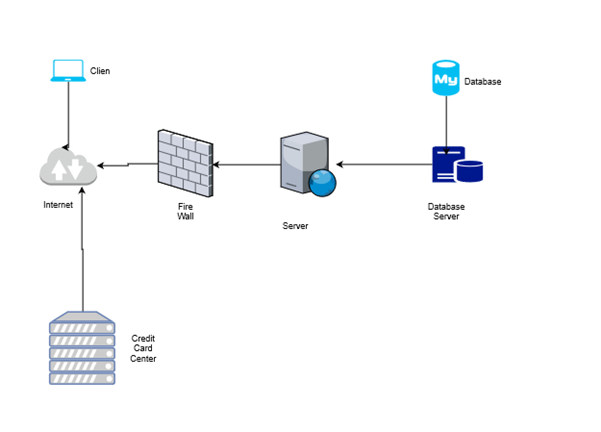
\includegraphics[width=13cm]{figures/sodo.png}
\caption{Biểu đồ hoạt động của thư viện}
\end{figure}


\section{Kết luận}
\subfile{sections/conclusion.tex}

\end{document}
